% Flow diagram draft (2026-10-22): what happens to an AI contribution.
\def\DoNotLoadEpstopdf{}
\documentclass[tikz,border=4pt]{standalone}
% Shared style for proposal figures (2026-10-22 visuals pass).
% Sized to print at 6.5 in (16.5 cm) wide; body text 9 pt sans, nothing below 8 pt.
\usepackage[T1]{fontenc}
\usepackage[scaled=0.95]{helvet}
\renewcommand{\familydefault}{\sfdefault}
\usepackage{xcolor}
\usetikzlibrary{arrows.meta,positioning,calc,patterns.meta}
\definecolor{cink}{HTML}{16191F}
\definecolor{cmuted}{HTML}{4B5563}
\definecolor{cslate}{HTML}{2F4858}
\definecolor{cslatefill}{HTML}{E9EFF3}
\definecolor{cbrass}{HTML}{7A5C12}
\definecolor{cbrassfill}{HTML}{F5EFDE}
\definecolor{cred}{HTML}{8C2F39}
\definecolor{credfill}{HTML}{F8E9EA}
\definecolor{cgreen}{HTML}{235C53}
\definecolor{cgreenfill}{HTML}{E3F0EC}
\definecolor{caudit}{HTML}{5B3A8E}
\definecolor{cauditfill}{HTML}{EFE9F6}
\definecolor{cghost}{HTML}{6B7280}
\definecolor{cghostfill}{HTML}{F3F4F6}
\tikzset{
  >={Triangle[length=5pt,width=4.5pt]},
  box/.style={draw, rounded corners=1.5pt, line width=0.8pt, align=center, inner sep=4pt, font=\fontsize{9}{11}\selectfont},
  sub/.style={font=\fontsize{8}{9.6}\selectfont, text=cmuted},
  ai/.style={box, draw=cbrass, fill=cbrassfill, text=cbrass},
  ver/.style={box, draw=cred, fill=credfill, text=cred},
  pipe/.style={box, draw=cslate, fill=cslatefill, text=cslate},
  prod/.style={box, draw=cslate, fill=cslate, text=white},
  person/.style={box, draw=cink, fill=white, text=cink},
  ghost/.style={box, draw=cghost, fill=cghostfill, text=cghost, dash pattern=on 3pt off 2pt},
  flow/.style={->, line width=0.8pt},
}

\begin{document}
\hyphenpenalty=10000
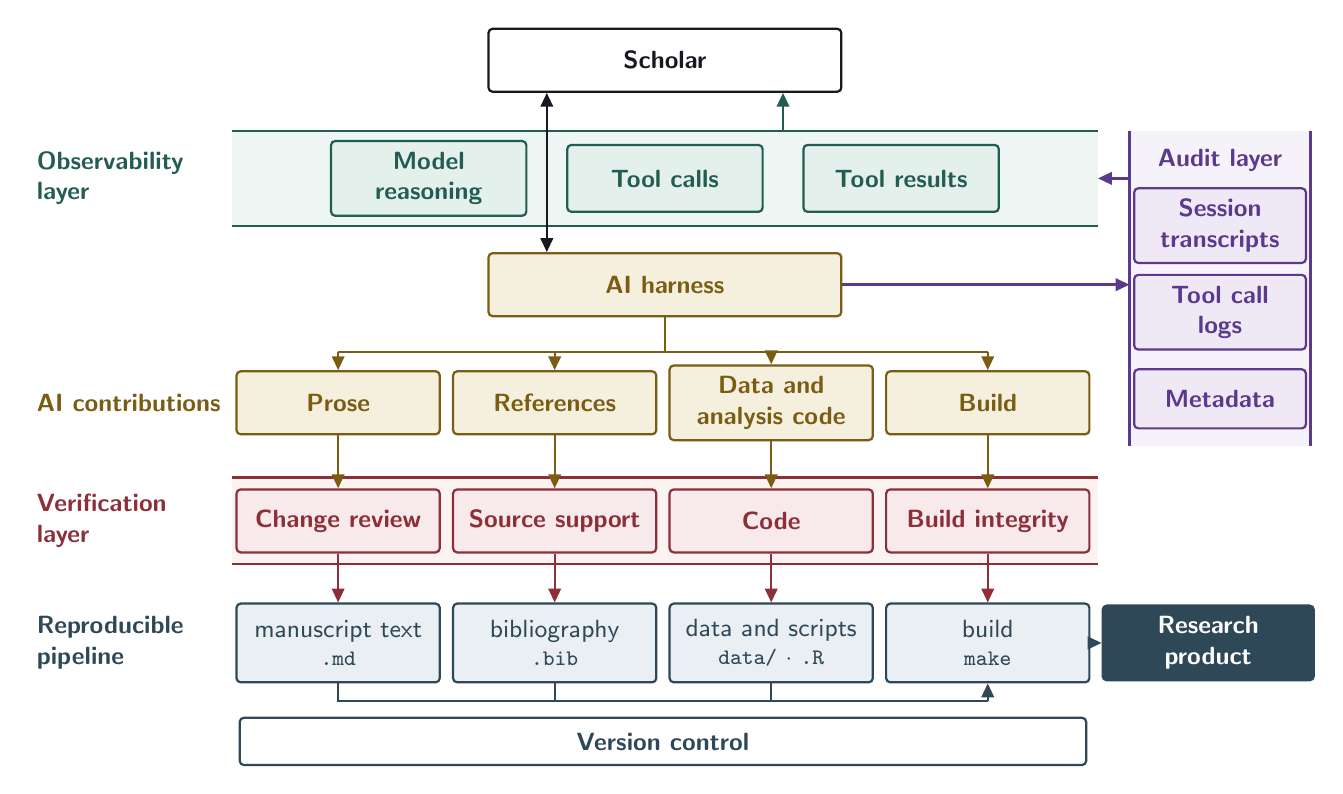
\begin{tikzpicture}
\tikzset{lab/.style={font=\fontsize{9}{11}\selectfont\bfseries, anchor=west, align=left, text width=2.4cm},
         col/.style={minimum width=2.5cm, minimum height=0.8cm, text width=2.3cm, font=\fontsize{9}{11}\selectfont\bfseries}}
\foreach \i in {0,1,2,3} {\pgfmathsetmacro{\x}{3.95+2.75*\i}\expandafter\xdef\csname cx\i\endcsname{\x}}
\node[person, col, minimum width=4.4cm, text width=4.2cm] (sch) at (8.1,2.85) {Scholar};
% observability band
\fill[cgreenfill!60!white] (2.6,0.75) rectangle (13.6,1.95);
\draw[cgreen, line width=0.8pt] (2.6,0.75) -- (13.6,0.75) (2.6,1.95) -- (13.6,1.95);
\node[lab, text=cgreen] at (0,1.35) {Observability layer};
\foreach \x/\t in {5.1/Model reasoning, 8.1/Tool calls, 11.1/Tool results} {
  \node[box, draw=cgreen, fill=cgreenfill, text=cgreen, minimum width=2.4cm, text width=2.2cm, minimum height=0.85cm, font=\fontsize{9}{11}\selectfont\bfseries] at (\x,1.35) {\t};
}
\draw[->, line width=0.9pt, cgreen] (9.6,1.95) -- (9.6,0 |- sch.south);
% audit band (alongside)
\fill[cauditfill!60!white] (14.0,1.95) rectangle (16.3,-2.05);
\draw[caudit, line width=0.8pt] (14.0,1.95) -- (14.0,-2.05) (16.3,1.95) -- (16.3,-2.05);
\node[font=\fontsize{9}{11}\selectfont\bfseries, text=caudit, anchor=north] at (15.15,1.85) {Audit layer};
\tikzset{aui/.style={box, draw=caudit, fill=cauditfill, text=caudit, minimum width=2.0cm, text width=1.9cm, minimum height=0.75cm, font=\fontsize{9}{11}\selectfont\bfseries}}
\node[aui] (a0) at (15.15,0.75) {Session transcripts};
\node[aui] (a1) at (15.15,-0.35) {Tool call\\logs};
\node[aui] (a2) at (15.15,-1.45) {Metadata};
\draw[->, line width=0.9pt, caudit] (14.0,1.35) -- (13.6,1.35);
\node[ai, col, minimum width=4.4cm, text width=4.2cm] (h) at (8.1,0) {AI harness};
\draw[<->, line width=0.8pt, cink] (6.6,0 |- sch.south) -- (6.6,0 |- h.north);
\draw[->, line width=0.9pt, caudit] (h.east) -- (14.0,0 |- h.east);
\draw[line width=0.8pt, cbrass] (h.south) -- ++(0,-0.45) coordinate (bus);
\draw[line width=0.8pt, cbrass] (3.95,-0.85) -- (12.2,-0.85);
\node[lab, text=cbrass] at (0,-1.5) {AI contributions};
\foreach \i/\t in {0/Prose, 1/References, 2/Data and\\analysis code, 3/Build} {
  \node[ai, col] (s\i) at (\csname cx\i\endcsname,-1.5) {\t};
  \draw[flow, cbrass] (\csname cx\i\endcsname,-0.85) -- (s\i.north);
}
\fill[credfill!60!white] (2.6,-2.45) rectangle (13.6,-3.55);
\draw[cred, line width=0.8pt] (2.6,-2.45) -- (13.6,-2.45) (2.6,-3.55) -- (13.6,-3.55);
\node[lab, text=cred] at (0,-3.0) {Verification layer};
\foreach \i/\t in {0/Change review, 1/Source support, 2/Code, 3/Build integrity} {
  \node[ver, col] (v\i) at (\csname cx\i\endcsname,-3.0) {\t};
  \draw[flow, cbrass] (s\i.south) -- (v\i.north);
}
\node[lab, text=cslate] at (0,-4.55) {Reproducible pipeline};
\foreach \i/\t/\u in {0/manuscript text/.md, 1/bibliography/.bib, 2/data and scripts/{data/ $\cdot$ .R}, 3/build/make} {
  \node[pipe, col, font=\fontsize{9}{11}\selectfont, minimum height=1.0cm] (p\i) at (\csname cx\i\endcsname,-4.55) {\t\\[-1pt]{\fontsize{8}{9.6}\selectfont\ttfamily \u}};
  \draw[flow, cred] (v\i.south) -- (p\i.north);
}
\node[prod, col, minimum width=2.6cm, text width=2.4cm] (rp) at (15.0,-4.55) {Research product};
\draw[line width=0.8pt, cslate] (p0.south) -- ++(0,-0.22) -- ($(p3.south)+(0,-0.22)$);
\foreach \i in {1,2} {\draw[line width=0.8pt, cslate] (p\i.south) -- ++(0,-0.22);}
\draw[flow, cslate] ($(p3.south)+(0,-0.22)$) -- (p3.south);
\draw[flow, cslate] (p3.east) -- (rp.west);
\node[pipe, minimum width=10.75cm, minimum height=0.6cm, font=\fontsize{9}{11}\selectfont\bfseries, fill=white] (vc) at (8.075,-5.8) {Version control};
\end{tikzpicture}
\end{document}
